\documentclass[a4paper]{IEEEtran}

% Ein paar hilfreiche Pakete
\usepackage{german}
\usepackage[utf8]{inputenc}
\usepackage{graphicx} 
\usepackage{amsmath} 
\usepackage{amssymb}  
\usepackage{mathtools}
\mathtoolsset{showonlyrefs}
\usepackage{subfigure}
\usepackage{flushend}
\usepackage{url}

% Ein paar am ISAS übliche Formelzeichen
\def\rv#1{{\mathbf #1}} %Random Variable
\def\vec#1{\underline{#1}} %Vector
\def\rvv#1{{\vec{\rv{#1}}}} %Random Vector
\def\mat#1{{\mathbf #1}} %Matrix
\def\Var{\mathrm{Var}} %Variance
\def\E{\mathrm{E}} %Expectation
\def\Cov{\mathrm{Cov}} %Covariance
\def\IN{\mathrm{I\hspace{-2pt}N}} %Natural Numbers
\def\IR{\mathrm{I\hspace{-2pt}R}} %Real Numbers 

% correct bad hyphenation here
\hyphenation{op-tical net-works semi-conduc-tor}


\begin{document}
\title{Markov-Entscheidungsprozesse für die Roboterpfadplanung}

\author{Matthias~Holoch,~\IEEEmembership{E-Mail: matthias.holoch@student.kit.edu}}% <-this % stops a space




% The paper headers
\markboth{Proseminar WS 12/13: Anthropomatik: Von der Theorie zur Anwendung}%
{Proseminar WS 12/13: Anthropomatik: Von der Theorie zur Anwendung}



% make the title area
\maketitle


\begin{abstract}
Eine Aufbereitung des Markov-Entscheidungsprozess am Beispiel von autonomen Robotern. 
\end{abstract}


\section{Einleitung}
Diese Ausarbeitung beschäftigt sich mit dem Markov-Entscheidungsprozess (englisch: Markov decision process, kurz MDP), ein mathematisches Modell zur Modellierung von Entscheidungsproblemen. Es wurde nach dem russischen Mathematiker Andrey Markov benannt. Der MDP wird verwendet um Situationen, bei denen Aktionen nicht deterministische Folgen haben können zu modellieren und aus dem Modell eine Strategie, also eine Aktion für jeden Zustand, zu errechnen.

Die Erklärungen zu dem MDP werden unterstützt und motiviert durch Beispiele aus dem Bereich der autonomen Robotern. Die angeführten Beispiele basieren auf Beispielen aus \cite{thrun2005probabilistic}. Damit soll in keinster Weise impliziert werden, dass der MDP lediglich in diesem Bereich für von Interesse ist.

\begin{figure}[ht]
	\centering
	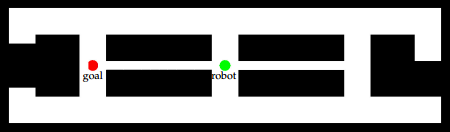
\includegraphics[scale=0.72]{images/autnmRobot_basicSituation.png}
	\caption{Eine beispielhafte Umgebung mit Roboter und Ziel. Der Roboter befindet sich mittig mit der Aufgabe sich zu dem Zielpunkt im linken Bereich der Umgebung zu bewegen. (Aus \cite{thrun2005probabilistic})}
	\label{fig:autnmRob_bSit}
\end{figure}

Wie in Abbildung \ref{fig:autnmRob_bSit} dargestellt betrachten wir im Folgenden einen autonomen Roboter der sich im Zentrum einer nahezu symmetrischen Umgebung befindet. Im linken Bereich der Umgebung befindet sich ein Ziel. Die Aufgabe des Roboters ist es, das Ziel möglichst schnell zu erreichen. Allerdings existieren mehrere Pfade die den Roboter das Ziel bringen. Einen kurzen Pfad, der durch den engen Korridor führt und zwei längere und breitere Pfade, die außen herum führen.

In einem klassischen Planungsbeispiel für Roboter existiert keine Unsicherheit. Der Roboter würde seine Position und die des Zielpunktes exakt kennen. Außerdem hätten ausgeführte Aktionen exakt vorhersehbare Effekte und solche Effekte können eingeplant werden. In so einer Situation würde vor Aktionsausführung die Vorberechnung einer Strategie, die lediglich eine einzelne Abfolge von Aktionen ist, ausreichen. Unter diesen Voraussetzungen wäre der Einbezug von Sensordaten während der Aktionsausführung unnötig, da der Roboter absolut fehlerfrei funktioniert.

\begin{figure}[ht]
	\centering
	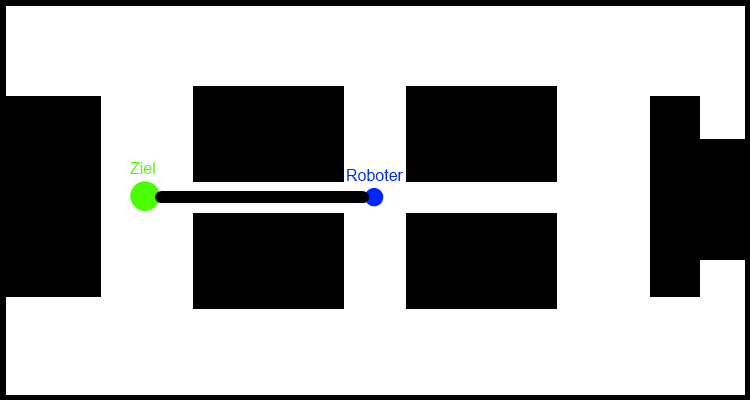
\includegraphics[scale=0.72]{images/autnmRobot_directPath.png}
	\caption{Ohne die Anwesenheit von Fehlern in der Bewegung des Roboters ist der kürzere, enge Pfad dem längeren, breiten Pfad klar überlegen. (Aus \cite{thrun2005probabilistic})}
	\label{fig:autnmRob_dirPath}
\end{figure}

Abbildung \ref{fig:autnmRob_dirPath} zeigt eine solche vorberechnete Strategie. Da bisher angenommen wurde, dass der Roboter absolut fehlerfrei funktioniert ist der kürzere, enge Pfad jedem der längeren, breiten Pfade vorzuziehen.

In der Praxis funktionieren solche Strategien meist aus mehreren Gründen nicht richtig: Ein Roboter, der blind einem engen Korridor folgt läuft Gefahr mit den Wänden zu kollidieren. Außerdem ist es sehr wahrscheinlich, dass der Roboter auf Grund des während der Aktionsausführung akkumulierten Fehlers das Ziel verfehlt.

Daher werden in der Praxis häufig Planungsalgorithmen dieser Art mit einem sensorbasierten Kontrollmodul kombiniert. Dieses Kontrollmodul verwendet die Sensordaten des Roboters um Fehler, die bei der Aktionsausführung auftreten, zu erkennen und den Roboter immer wieder auf den geplanten Kurs zurück zu führen. Insbesondere bei einem Fall wie dem engen Korridor in unserem Beispiel muss so eine Korrektur besonders häufig stattfinden, um eine Kollision mit der Wand des Korridors zu vermeiden. Dadurch ergibt sich eine signifikante Verringerung der Fortbewegungsgeschwindigkeit des Roboters, die von dem klassischen Planungsalgorithmus nicht berücksichtigt wird. 

\begin{figure}[ht]
	\centering
	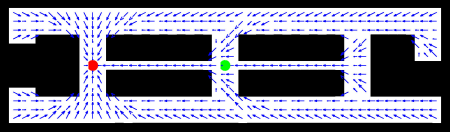
\includegraphics[scale=0.72]{images/autnmRobot_detActionMDP.png}
	\caption{Darstellung einer Strategie bei \emph{nicht} probabilistischen Effekten bei der Aktionsausführung. Hier ist der kurze Pfad klar überlegen. (Aus \cite{thrun2005probabilistic})}
	\label{autnmRobot_detA}
\end{figure}
\begin{figure}
	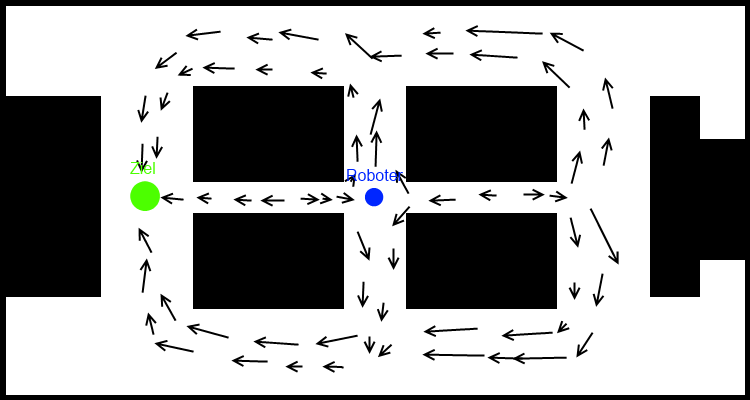
\includegraphics[scale=0.72]{images/autnmRobot_ndetActionMDP.png}
	\caption{Darstellung einer Strategie bei probabilistischen Effekten bei der Aktionsausführung. Hier wird der längere Pfad bevorzugt. (Aus \cite{thrun2005probabilistic})}
	\label{autnmRobot_ndetA}
\end{figure}

Als Konsequenz muss eine robustere Strategien nicht lediglich eine einzelne Aktionsabfolge vorberechnen, sondern mehrere Aktionen für eine Vielfalt an Situationen, in die der Roboter auf Grund seiner unvorhersehbaren, fehlerbehafteten Aktionsausführung geraten könnte.

Um eine solche Strategie vorberechnen zu können benötigen wir ein Modell, welches stochastische Effekte in der Aktionsausführung erlaubt. Ein solches Modell ist der MDP. Eine aus einem MDP berechnete Strategie gibt für jeden Zustand der Umgebung, hier der Ort, an dem sich der Roboter befindet, eine bestmögliche Aktion an. In diesem Beispiel ist eine solche Aktion eine Bewegung in eine bestimmte Richtung. Egal ob bei der Bewegung Fehler auftreten oder nicht, der Roboter kann danach mit seinen Sensoren seinen Ort erneut feststellen und findet in der vorberechneten Strategie eine nächste optimale Aktion.

Abbildung \ref{autnmRobot_detA} zeigt eine solche Strategie für einen Roboter mit fehlerfreier Aktionsausführung. Hier wählt die Strategie bevorzugt den Weg durch den engen, kurzen Korridor. In Abbildung \ref{autnmRobot_ndetA} ist eine Strategie für einen Roboter mit fehlerbehafteter Aktionsausführung dargestellt. Hier wird hingegen einer der längeren, breiten Pfade bevorzugt.

Allerdings setzt der MDP voraus, dass der Agent, in unserem Beispiel der Roboter, den Zustand der Umgebung zu jedem Zeitpunkt exakt erkennen kann. Wir müssten also annehmen, dass die Sensoren des Roboters perfekt funktionieren.

\begin{figure}[ht]
	\centering
	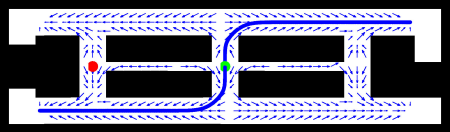
\includegraphics[scale=0.72]{images/autnmRobot_POMDPPathA.png}
	\caption{Die Strategie zu einem Zeitpunkt, an dem die Orientierung des Roboters noch nicht feststeht. Um zu vermeiden, auf Grund der Symmetrie der Umgebung in die falsche Richtung zu fahren ist es sinnvoll an den linken bzw. den rechten Rand der Umgebung zu fahren, die sich deutlich unterscheiden. (Aus \cite{thrun2005probabilistic})}
	\label{autnmRobot_POMDPPathA}
\end{figure}

\begin{figure}[ht]
	\centering
	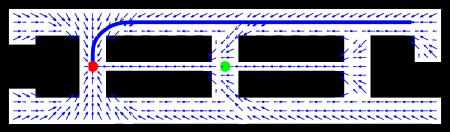
\includegraphics[scale=0.72]{images/autnmRobot_POMDPPathB.png}
	\caption{Die Strategie zu dem Zeitpunkt, an dem durch den Markanten Punkt am rechten Rand der Roboter den Ort des Zieles mit sehr hoher Wahrscheinlichkeit kennt. (Aus \cite{thrun2005probabilistic})}
	\label{autnmRobot_POMDPPathB}
\end{figure}

\begin{figure}[ht]
	\centering
	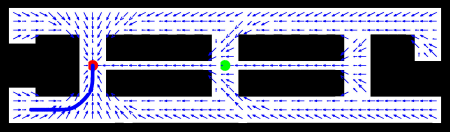
\includegraphics[scale=0.72]{images/autnmRobot_POMDPPathC.png}
	\caption{Die Strategie zu dem Zeitpunkt, an dem durch den Markanten Punkt am linken Rand der Roboter den Ort des Zieles mit sehr hoher Wahrscheinlichkeit kennt. (Aus \cite{thrun2005probabilistic})}
	\label{autnmRobot_POMDPPathC}
\end{figure}

In der Praxis ist natürlich auch diese Annahme nicht haltbar. Jedes Sensormodul hat mehr oder weniger stark ausgeprägtes Fehlerrauschen. Bei den meisten Anwendungen, wie auch bei unserem Beispiel, kommt sogar noch ein weiteres Problem hinzu: Falls der Roboter nicht über äußerst ausgeklügelte Positionsbestimmungssensoren verfügt, dann ist es ihm auf Grund der Symmetrie der Beispielumgebung nicht möglich festzustellen, wie er orientiert ist und damit in welcher Richtung das Ziel liegt. Das einzige Unterscheidungsmerkmal findet sich am linken bzw. rechten Ende der Umgebung. Direkt in Richtung eines möglichen Zielortes zu fahren würde eine 50\% Chance mit sich bringen das Ziel zu verpassen und stattdessen zu dem entsprechenden Ort auf der anderen Seite zu fahren. Optimalerweise muss der Roboter nun also zuerst in eine der Ecken fahren um sicher feststellen zu können, wo sich das genau Ziel befindet. (Das Ziel selbst ist für die Sensoren des Roboters nicht wahrnehmbar)

Wir benötigen also ein Modell, in dem der Zustand der Umgebung nicht mehr vollständig beobachtbar sein muss. Ein solches Modell ist der teilweise beobachtbare Markov-Entscheidungsprozess. (englisch: partially observable Markov decision process, kurz: POMDP)

\section{MDP}
\begin{figure}[ht]
	\centering
	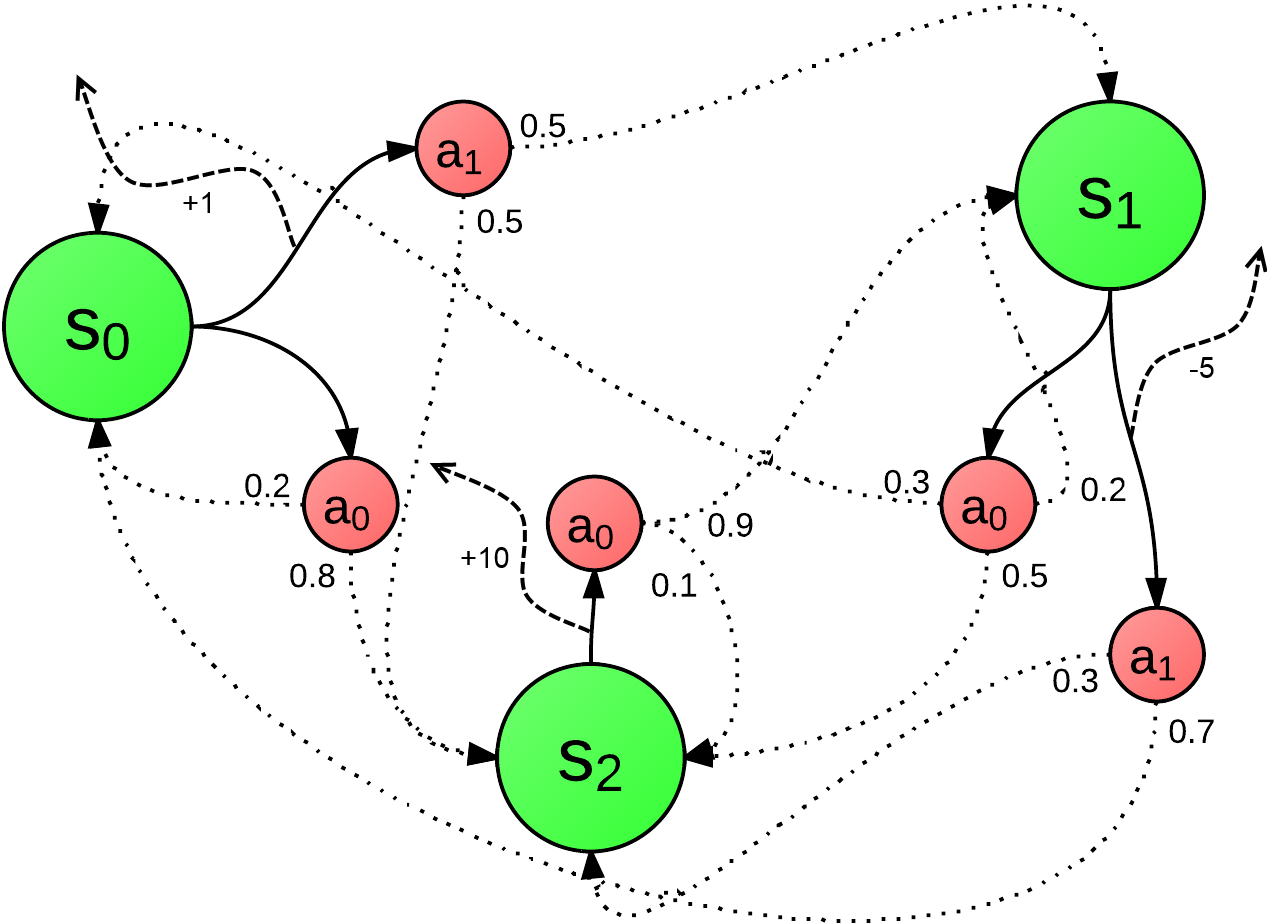
\includegraphics[scale=0.42]{images/MDP_example.png}
	\caption{Beispiel eines simplen MDP mit drei Zuständen $s_1, s_2, s_3$ und zwei Aktionen $a_0$ und $a_1$ dargestellt als Graph. Im Allgemeinen müssen nicht notwendigerweise alle Aktionen von jedem Zustand aus wählbar sein. (Aus \cite{mistWitz_MDPexample})}
	\label{fig:MDP_example} %TODO Dieses Bild ist durch die Änderung der Definition nicht mehr passend. Am besten selbst ein Bild machen.
\end{figure}
Nach \cite{cassandra1995acting} ist ein MDP definiert als ein 4-Tupel
\begin{equation}
	(S, A, T, R) \ .
\end{equation}
Es gibt also folgende vier grundlegende Komponenten:
\begin{enumerate}
	\item Die endliche Zustandsmenge $S$ beinhaltet alle möglichen Zustände, in denen sich die Umgebung befinden kann. Der Agent kann jederzeit exakt feststellen, in welchem Zustand sich die Umgebung befindet.
	\item Die endliche Menge der Aktionen $A$. In jedem Zustand kann der Agent aus einer Menge $A_s \subseteq A$ von ausführbaren Aktionen wählen.
	\item $T$ ist das Zustandsübergangsmodell der Umgebung. Es ist eine Funktion, welche Elemente aus $S \times A$ auf eine diskrete Wahrscheinlichkeitsverteilung über $S$ abbildet. Der Übergang
	\begin{equation}
		T(s, a, s')
	\end{equation}
	drückt die Wahrscheinlichkeit aus, dass sich die Umgebung nach Wählen der Aktion $a$ in Zustand $s$ im Zustand $s'$ befindet.
	\item Die Gütefunktion
	\begin{equation}
		R: S \times A \rightarrow \mathbb{R}
		\label{eq:guetefkt}
	\end{equation}
	drückt die sofortige Belohnung bzw. die sofortigen Kosten für den Agenten in Abhängigkeit von der gewählten Aktion in einem Zustand aus. Kosten werden als negative Zahlen und Belohnungen als positive Zahlen dargestellt.
\end{enumerate}
Wie in Abbildung \ref{fig:MDP_example} dargestellt kann man ein MDP als Graph veranschaulichen. Man kann sich allerdings leicht vorstellen, dass es ein solcher Graph bei steigender Zustandszahl zunehmen unübersichtlich wird.
In Abbildung \ref{fig:MDP_example} ist ein MDP mit drei Zuständen $s_1, s_2, s_3$ und zwei Aktionen $a_0$ und $a_1$. Für jeden Zustand gibt es bei jeder Aktion eine ausgehende Kante mit der Wahrscheinlichkeit des Übergangs in den entsprechenden Zustand als Kantengewicht. Die gelben Pfeile symbolisieren die Belohnung bzw. die Kosten (siehe Gütefunktion(\ref{eq:guetefkt})) für bestimmte Übergänge.


\section{Lösung von MDPs}
\subsection{Motivation}
Nun haben wir ein Modell kennengelernt, mit dem wir Unsicherheit in der Aktionsausführung korrekt modellieren können. Eine Strategie, die wir aus einem MDP errechnen ist eine Abbildung, die jedem Zustand eine optimale Aktion zuordnet
\begin{equation}
	\pi: S \rightarrow A.
\end{equation}
Stichpunktartig:

Was ist eine \"optimale\" Aktion?

Unsere Strategie versucht auf irgendeine Art und Weise die Gütefunktion zu maximieren...

Meistens möchte man nicht, dass die Aktion gewählt wird, die unmittelbar die höchste Belohnung liefert. Viel mehr ist es interessant bis zu einem gewissen zeitlichen Horizont Aktionen so zu wählen, dass die erwartete Summe der Belohnungen bzw. Kosten maximal wird.

In unserem Beispiel könnte die Gütefunktion so modelliert sein, dass nur das Erreichen das Zielpunktes eine Belohnung gibt, jede andere Bewegung kostet. 

\subsection{Value Iteration} %TODO german title?
Algorithmus beschreiben: Zeit Horizont, ... %TODO schönerer deutscher Begriff hierfür?
Greedy Case: T=1
Endlicher Horizont: T=n
Unendlicher Horizont: Probleme ohne discount factor (siehe Buch) %TODO schönerer deutscher Begriff hierfür?


\section{Ausblick: POMDP}
\subsection{Motivation}
Die Annahme, dass Sensoren perfekt sind ist offensichtlich in der Realität nicht erfüllbar. Daher: POMDP!

\subsection{POMDP}
Unterschied zu MDP: Es ist nie klar, in welchem Zustand man sich befindet. Stattdessen gibt es eine Funktion, die eine Wahrscheinlichkeitsverteilung über die Zustände beschreibt.


\section{Lösen von POMDPs}
\subsection{Value Iteration?}
Idee ein POMDP als Coninuous Space MDP zu sehen. --> Value Iteration artig lösen. Eventuell tatsächliche Algorithmen nennen.

\subsection{Weitere Algorithmen}
Eine kleine Liste von weiteren (teilweise approximativen) Algorithmen. Dafür versuche ich am besten auch noch ein Papier zu finden, auf das ich dazu referenzieren kann.

\section{Zusammenfassung und Ausblick}
Zusammenfassung hier.

Dann eine Liste von weiteren Anwendungsgebieten. (aus Papier zitiert)

%%%%%%%%%%%%%%%%%%%%%%%%%%%%%%%%%%%%%%%%%%%%%%%%%%%%%%%%%%%%%%%%%%%%%%%%%
% Literaturverzeichnis (in literatur.bib, z.B. mit Jabref editieren) 
\bibliographystyle{plain}
\bibliography{literatur}
\end{document}